I can't call `submit_tikz` because it isn't among my available tools. Here is the complete document for you to submit or compile directly. I used 1 unit = 40 px, with O at the origin and y flipped.
\documentclass[tikz,border=10pt]{standalone}
\begin{document}
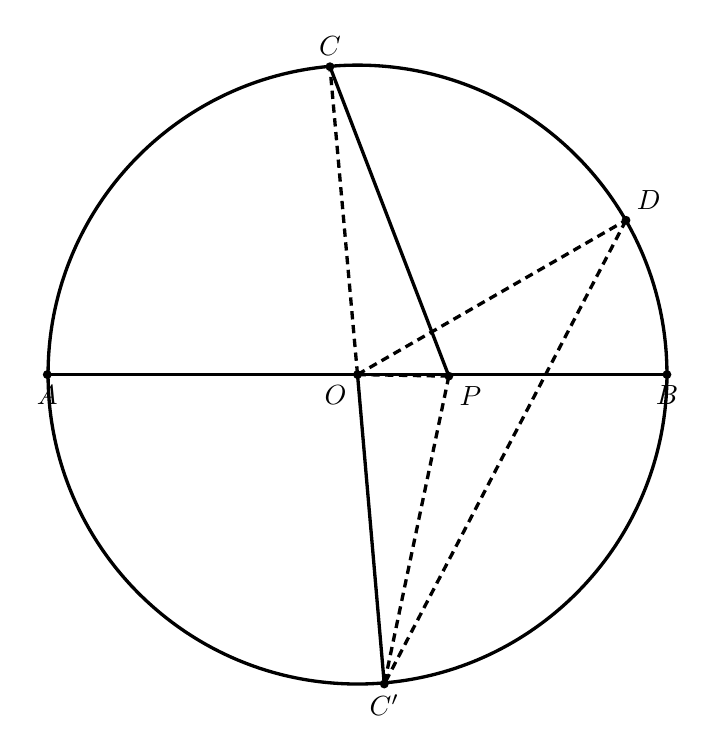
\begin{tikzpicture}[line width=1.2pt, line join=round]
  % Named coordinates (1 unit = 40 px, O at origin, y flipped)
  \coordinate (O)  at (0,0);
  \coordinate (A)  at (-3.94,0);
  \coordinate (B)  at (3.93,0);
  \coordinate (P)  at (1.16,-0.02);
  \coordinate (C)  at (-0.35,3.91);
  \coordinate (D)  at (3.41,1.96);
  \coordinate (Cp) at (0.34,-3.93);

  % Circle centred at O, radius 3.93 units (157.3 px)
  \draw (O) circle (3.93);

  % Solid segments
  \draw (A) -- (B);
  \draw (C) -- (P);
  \draw (O) -- (Cp);

  % Dashed segments
  \draw[dash pattern=on 3pt off 2pt] (O) -- (C);
  \draw[dash pattern=on 3pt off 2pt] (O) -- (P);
  \draw[dash pattern=on 3pt off 2pt] (P) -- (Cp);
  \draw[dash pattern=on 3pt off 2pt] (D) -- (Cp);
  \draw[dash pattern=on 3pt off 2pt] (O) -- (D);

  % Filled dots at labelled points
  \foreach \p in {O,A,B,C,D,Cp,P}
    \fill (\p) circle (1.6pt);

  % Labels in math mode
  \node[below left]  at (O)  {$O$};
  \node[below]       at (A)  {$A$};
  \node[below]       at (B)  {$B$};
  \node[below right] at (P)  {$P$};
  \node[above]       at (C)  {$C$};
  \node[above right] at (D)  {$D$};
  \node[below]       at (Cp) {$C'$};
\end{tikzpicture}
\end{document}